\documentclass[border=2pt]{standalone}
\usepackage{tikz}
\usetikzlibrary{arrows.meta,plotmarks}
\begin{document}
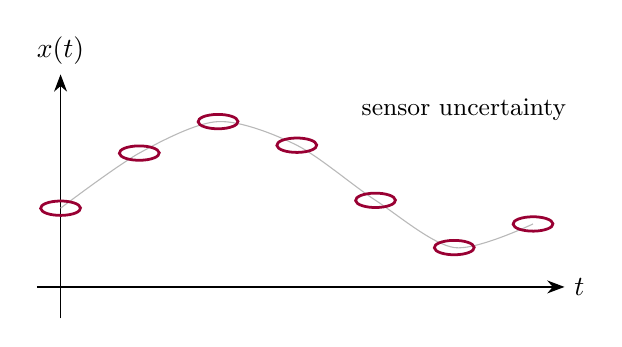
\begin{tikzpicture}
  \draw[-{Stealth[length=2.2mm]}] (-.3,0) -- (6.4,0) node[right] {$t$};
  \draw[-{Stealth[length=2.2mm]}] (0,-.4) -- (0,2.7) node[above] {$x(t)$};
  \draw[gray!55] plot[smooth] coordinates {(0,1) (1,1.7) (2,2.1) (3,1.8) (4,1.1) (5,.5) (6,.8)};
  \tikzset{every mark/.append style={xscale=1.8,yscale=.65,rotate=25,draw=purple!80!black,line width=1pt}}
  \draw[mark size=4pt]
    plot[only marks,mark=o] coordinates {(0,1) (1,1.7) (2,2.1) (3,1.8) (4,1.1) (5,.5) (6,.8)};
  \node[anchor=west,font=\small] at (3.7,2.25) {sensor uncertainty};
\end{tikzpicture}
\end{document}
